% Created by tikzDevice version 0.12.6 on 2026-05-17 18:10:18
% !TEX encoding = UTF-8 Unicode
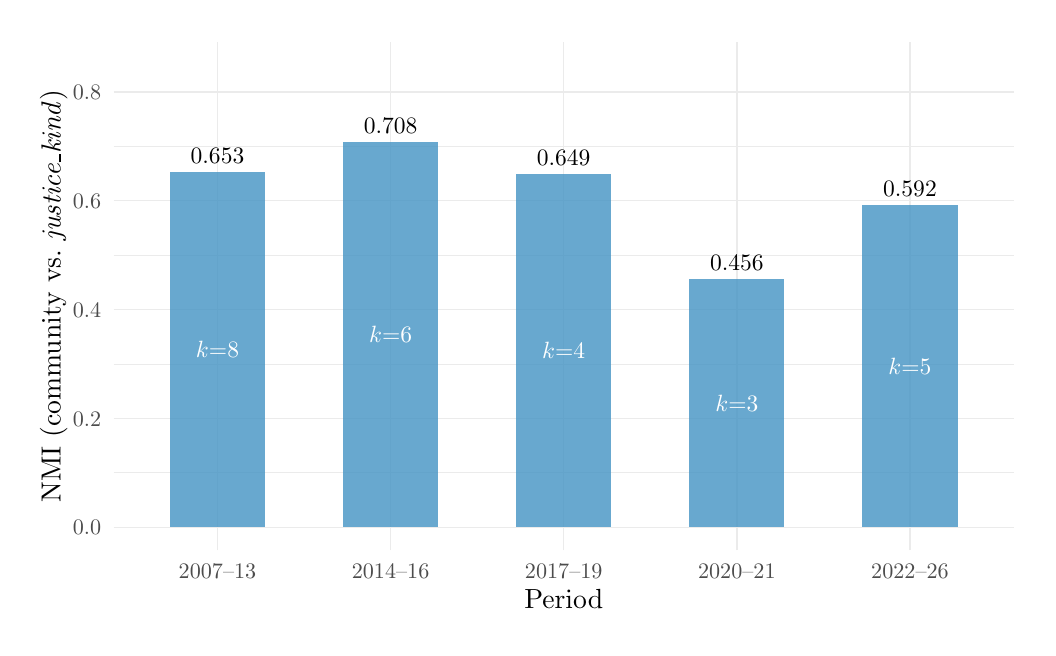
\begin{tikzpicture}[x=1pt,y=1pt]
\definecolor{fillColor}{RGB}{255,255,255}
\path[use as bounding box,fill=fillColor,fill opacity=0.00] (0,0) rectangle (361.35,216.81);
\begin{scope}
\path[clip] (  0.00,  0.00) rectangle (361.35,216.81);
\definecolor{fillColor}{RGB}{255,255,255}

\path[fill=fillColor] (  0.00,  0.00) rectangle (361.35,216.81);
\end{scope}
\begin{scope}
\path[clip] ( 31.05, 27.90) rectangle (356.35,211.81);
\definecolor{drawColor}{gray}{0.92}

\path[draw=drawColor,line width= 0.3pt,line join=round] ( 31.05, 55.93) --
	(356.35, 55.93);

\path[draw=drawColor,line width= 0.3pt,line join=round] ( 31.05, 95.27) --
	(356.35, 95.27);

\path[draw=drawColor,line width= 0.3pt,line join=round] ( 31.05,134.61) --
	(356.35,134.61);

\path[draw=drawColor,line width= 0.3pt,line join=round] ( 31.05,173.95) --
	(356.35,173.95);

\path[draw=drawColor,line width= 0.5pt,line join=round] ( 31.05, 36.26) --
	(356.35, 36.26);

\path[draw=drawColor,line width= 0.5pt,line join=round] ( 31.05, 75.60) --
	(356.35, 75.60);

\path[draw=drawColor,line width= 0.5pt,line join=round] ( 31.05,114.94) --
	(356.35,114.94);

\path[draw=drawColor,line width= 0.5pt,line join=round] ( 31.05,154.28) --
	(356.35,154.28);

\path[draw=drawColor,line width= 0.5pt,line join=round] ( 31.05,193.62) --
	(356.35,193.62);

\path[draw=drawColor,line width= 0.5pt,line join=round] ( 68.59, 27.90) --
	( 68.59,211.81);

\path[draw=drawColor,line width= 0.5pt,line join=round] (131.14, 27.90) --
	(131.14,211.81);

\path[draw=drawColor,line width= 0.5pt,line join=round] (193.70, 27.90) --
	(193.70,211.81);

\path[draw=drawColor,line width= 0.5pt,line join=round] (256.26, 27.90) --
	(256.26,211.81);

\path[draw=drawColor,line width= 0.5pt,line join=round] (318.82, 27.90) --
	(318.82,211.81);
\definecolor{fillColor}{RGB}{67,147,195}

\path[fill=fillColor,fill opacity=0.80] ( 51.38, 36.26) rectangle ( 85.79,164.70);

\path[fill=fillColor,fill opacity=0.80] (113.94, 36.26) rectangle (148.35,175.52);

\path[fill=fillColor,fill opacity=0.80] (176.50, 36.26) rectangle (210.90,163.91);

\path[fill=fillColor,fill opacity=0.80] (239.05, 36.26) rectangle (273.46,125.95);

\path[fill=fillColor,fill opacity=0.80] (301.61, 36.26) rectangle (336.02,152.70);
\definecolor{drawColor}{RGB}{0,0,0}

\node[text=drawColor,anchor=base,inner sep=0pt, outer sep=0pt, scale=  0.85] at ( 68.59,167.64) {0.653};

\node[text=drawColor,anchor=base,inner sep=0pt, outer sep=0pt, scale=  0.85] at (131.14,178.46) {0.708};

\node[text=drawColor,anchor=base,inner sep=0pt, outer sep=0pt, scale=  0.85] at (193.70,166.85) {0.649};

\node[text=drawColor,anchor=base,inner sep=0pt, outer sep=0pt, scale=  0.85] at (256.26,128.89) {0.456};

\node[text=drawColor,anchor=base,inner sep=0pt, outer sep=0pt, scale=  0.85] at (318.82,155.64) {0.592};
\definecolor{drawColor}{RGB}{255,255,255}

\node[text=drawColor,anchor=base,inner sep=0pt, outer sep=0pt, scale=  0.85] at ( 68.59, 97.54) {$k{=}8$};

\node[text=drawColor,anchor=base,inner sep=0pt, outer sep=0pt, scale=  0.85] at (131.14,102.95) {$k{=}6$};

\node[text=drawColor,anchor=base,inner sep=0pt, outer sep=0pt, scale=  0.85] at (193.70, 97.15) {$k{=}4$};

\node[text=drawColor,anchor=base,inner sep=0pt, outer sep=0pt, scale=  0.85] at (256.26, 78.16) {$k{=}3$};

\node[text=drawColor,anchor=base,inner sep=0pt, outer sep=0pt, scale=  0.85] at (318.82, 91.54) {$k{=}5$};
\end{scope}
\begin{scope}
\path[clip] (  0.00,  0.00) rectangle (361.35,216.81);
\definecolor{drawColor}{gray}{0.30}

\node[text=drawColor,anchor=base east,inner sep=0pt, outer sep=0pt, scale=  0.80] at ( 26.55, 33.50) {0.0};

\node[text=drawColor,anchor=base east,inner sep=0pt, outer sep=0pt, scale=  0.80] at ( 26.55, 72.84) {0.2};

\node[text=drawColor,anchor=base east,inner sep=0pt, outer sep=0pt, scale=  0.80] at ( 26.55,112.18) {0.4};

\node[text=drawColor,anchor=base east,inner sep=0pt, outer sep=0pt, scale=  0.80] at ( 26.55,151.52) {0.6};

\node[text=drawColor,anchor=base east,inner sep=0pt, outer sep=0pt, scale=  0.80] at ( 26.55,190.86) {0.8};
\end{scope}
\begin{scope}
\path[clip] (  0.00,  0.00) rectangle (361.35,216.81);
\definecolor{drawColor}{gray}{0.30}

\node[text=drawColor,anchor=base,inner sep=0pt, outer sep=0pt, scale=  0.80] at ( 68.59, 17.89) {2007--13};

\node[text=drawColor,anchor=base,inner sep=0pt, outer sep=0pt, scale=  0.80] at (131.14, 17.89) {2014--16};

\node[text=drawColor,anchor=base,inner sep=0pt, outer sep=0pt, scale=  0.80] at (193.70, 17.89) {2017--19};

\node[text=drawColor,anchor=base,inner sep=0pt, outer sep=0pt, scale=  0.80] at (256.26, 17.89) {2020--21};

\node[text=drawColor,anchor=base,inner sep=0pt, outer sep=0pt, scale=  0.80] at (318.82, 17.89) {2022--26};
\end{scope}
\begin{scope}
\path[clip] (  0.00,  0.00) rectangle (361.35,216.81);
\definecolor{drawColor}{RGB}{0,0,0}

\node[text=drawColor,anchor=base,inner sep=0pt, outer sep=0pt, scale=  1.00] at (193.70,  6.94) {Period};
\end{scope}
\begin{scope}
\path[clip] (  0.00,  0.00) rectangle (361.35,216.81);
\definecolor{drawColor}{RGB}{0,0,0}

\node[text=drawColor,rotate= 90.00,anchor=base,inner sep=0pt, outer sep=0pt, scale=  1.00] at ( 11.89,119.85) {NMI (community vs.\ \emph{justice\_kind})};
\end{scope}
\end{tikzpicture}
